\chapter{Теоретическое исследование и архитектура}\label{arch}

\section{Поиск вероятностных лазеек}\label{arch:rbs}

\subsection{Схема алгоритма}\label{arch:rbs:schema}

В данной главе описаны алгоритмы поиска вероятностных лазеек.
Для поиска вероятностных лазеек применяются эволюционные алгоритмы, а именно, (1 + 1) и (q + h)
алгоритмы~\cite{bib:ea},~\cite{bib:ga}. Для полного описания теоретической схемы поиска 
вероятностных лазеек необходимо определить особь, фитнес-функцию, а также операторы скрещивания, 
мутации и отбора.

\textbf{Особью} во всех реализованных схемах поиска вероятностных лазеек является битовая маска
$\overline{B}$, соответствующая множеству переменных $B$, включенных в лазейку.

\textbf{Фитнес функция}. В фитнес-функции используется аппроксимация значения $\rho$, формально 
определенная уравнением \ref{overview:rho-hat}, так как такой
подход позволяет вычислять его с достаточно высокой точностью, а главное --- быстро. В качестве
алгоритма $A$ используется \textit{вывод последствий, или unit propagation (UP)}, эффективно реализованный
в рамках решателя Minisat~\cite{bib:minisat}. Данный алгоритм с точки зрения решателя не является
полным, но имеет полиномиальное время работы.

Используется фитнес функция, описанная в TBD-REF. Её преимущество заключается в том, что она помимо 
максимизации $\hat{\rho}$-значения лазейки минимизирует её размер. Максимизация $\hat{\rho}$-значения 
достигается первой частью функции:
\[
    G_{C}\left(\overline{B}\right) = (1 - \hat{\rho}_B) \cdot 2^{\omega |V|},
\]
где $C$ --- формула \ref{overview:formula}, $V$ --- множество переменных в формуле, $w \in (0, 1]$
-- константа. Минимизация размера лазейки обеспечивается второй частью функции:
\[
    f_{C, \min{|B|}} = \hat{\rho}_B \cdot 2^{|B|}.
\]
Действительно, при относительно близких значениях $\rho$ большое влияние на функцию будет оказывать
размер лазейки $B$. Итоговая фитнес функция выглядит следующим образом:
\begin{equation}
    f_{C}\left(\overline{B}\right) = \hat{\rho}_B \cdot 2^{|B|} + (1 - \hat{\rho}_B) \cdot 2^{\omega |V|}.
    \label{arch:fitness}
\end{equation}

\textbf{Операторы}
В качестве основного оператора мутации был выбран зарекоммендовавший себя в TBD-REF оператор 
\textsc{Doerr}~\cite{bib:doerr}. В процессе разработки также использовался равномерный оператор
мутации, однако результаты, которые он показывал, стабильно хуже результатов \textsc{Doerr} на
всех примерах, поэтому он был отброшен, однако доступен в конфигурации. Реализованы операторы
одноточечного и двуточечного скрещивания. Генетический алгоритм $(\mu + \lambda)$ был
реализован аналогично схеме, предложенной в TBD-REF.

\subsection{Эффективный вывод последствий}\label{arch:rbs:prop}

Основным потребителем ресурсов в описанной схеме поиска вероятностных лазеек является алгоритм
вывода последствий, реализованный в Minisat~\cite{bib:minisat}. Поэтому оптимизация этого алгоритма
и разработка новых подходов является крайне важной задачей для достижения высокой производительности.

\textit{Выборка}\label{arch:rbs:prop:sampling}. Заметим, что для достаточно маленьких $B$ имеет
смысл производить полный перебор множества $\hat{B}$ при вычислении $\hat{\rho}$. Во-первых,
это обеспечит точное значение $\hat{\rho} = \rho$, во-вторых, реализация перебора всех подстановок
(то есть, перебора всех возможных назначений переменных из набора в $\mathcal{B}$, что эквивалентно
перебору всех чисел от $0$ до $2^{|B|} - 1$ в двоичной записи) точно будет работать не медленнее,
чем случайный перебор $2^{|B|}$ подстановок, так как не пользуется геренацией случайных чисел и
делает строго меньше операций засчет того, что не на каждом шаге модифицируются все значения подстановки.

Данное наблюдение создает необходимость в абстракции от типа выборки. Для этого был создан интерфейс
\textsc{Search}, а также следующие реализации:
\begin{itemize}
    \item \textsc{FullSearch} --- перебор всех возможных $\hat{b} \in \hat{B}$.
    \item \textsc{RandomSearch} --- перебор $N$ случайных подстановок из $\hat{B}$.
    \item \textsc{UniqueSearch} --- перебор $N$ уникальных случайных подстановок из $\hat{B}$.
    \item \textsc{CartesianSearch} --- перебор всех подстановок из декартового произведения
        нескольких наборов подстановок, необходимая для реализации некоторых стратегий 
        (см. Главу \ref{arch:solve}).
\end{itemize}

На рисунке \ref{arch:rbs:prop:search-img} представлена схема наследования интерфейса \textsc{Search}.
Далее в таблице \ref{arch:rbs:prop:search-def} описаны методы интерфейса.

\begin{figure}[H]
    \caption{Интерфейс \textsc{Search} и его реализации}
    \centering
    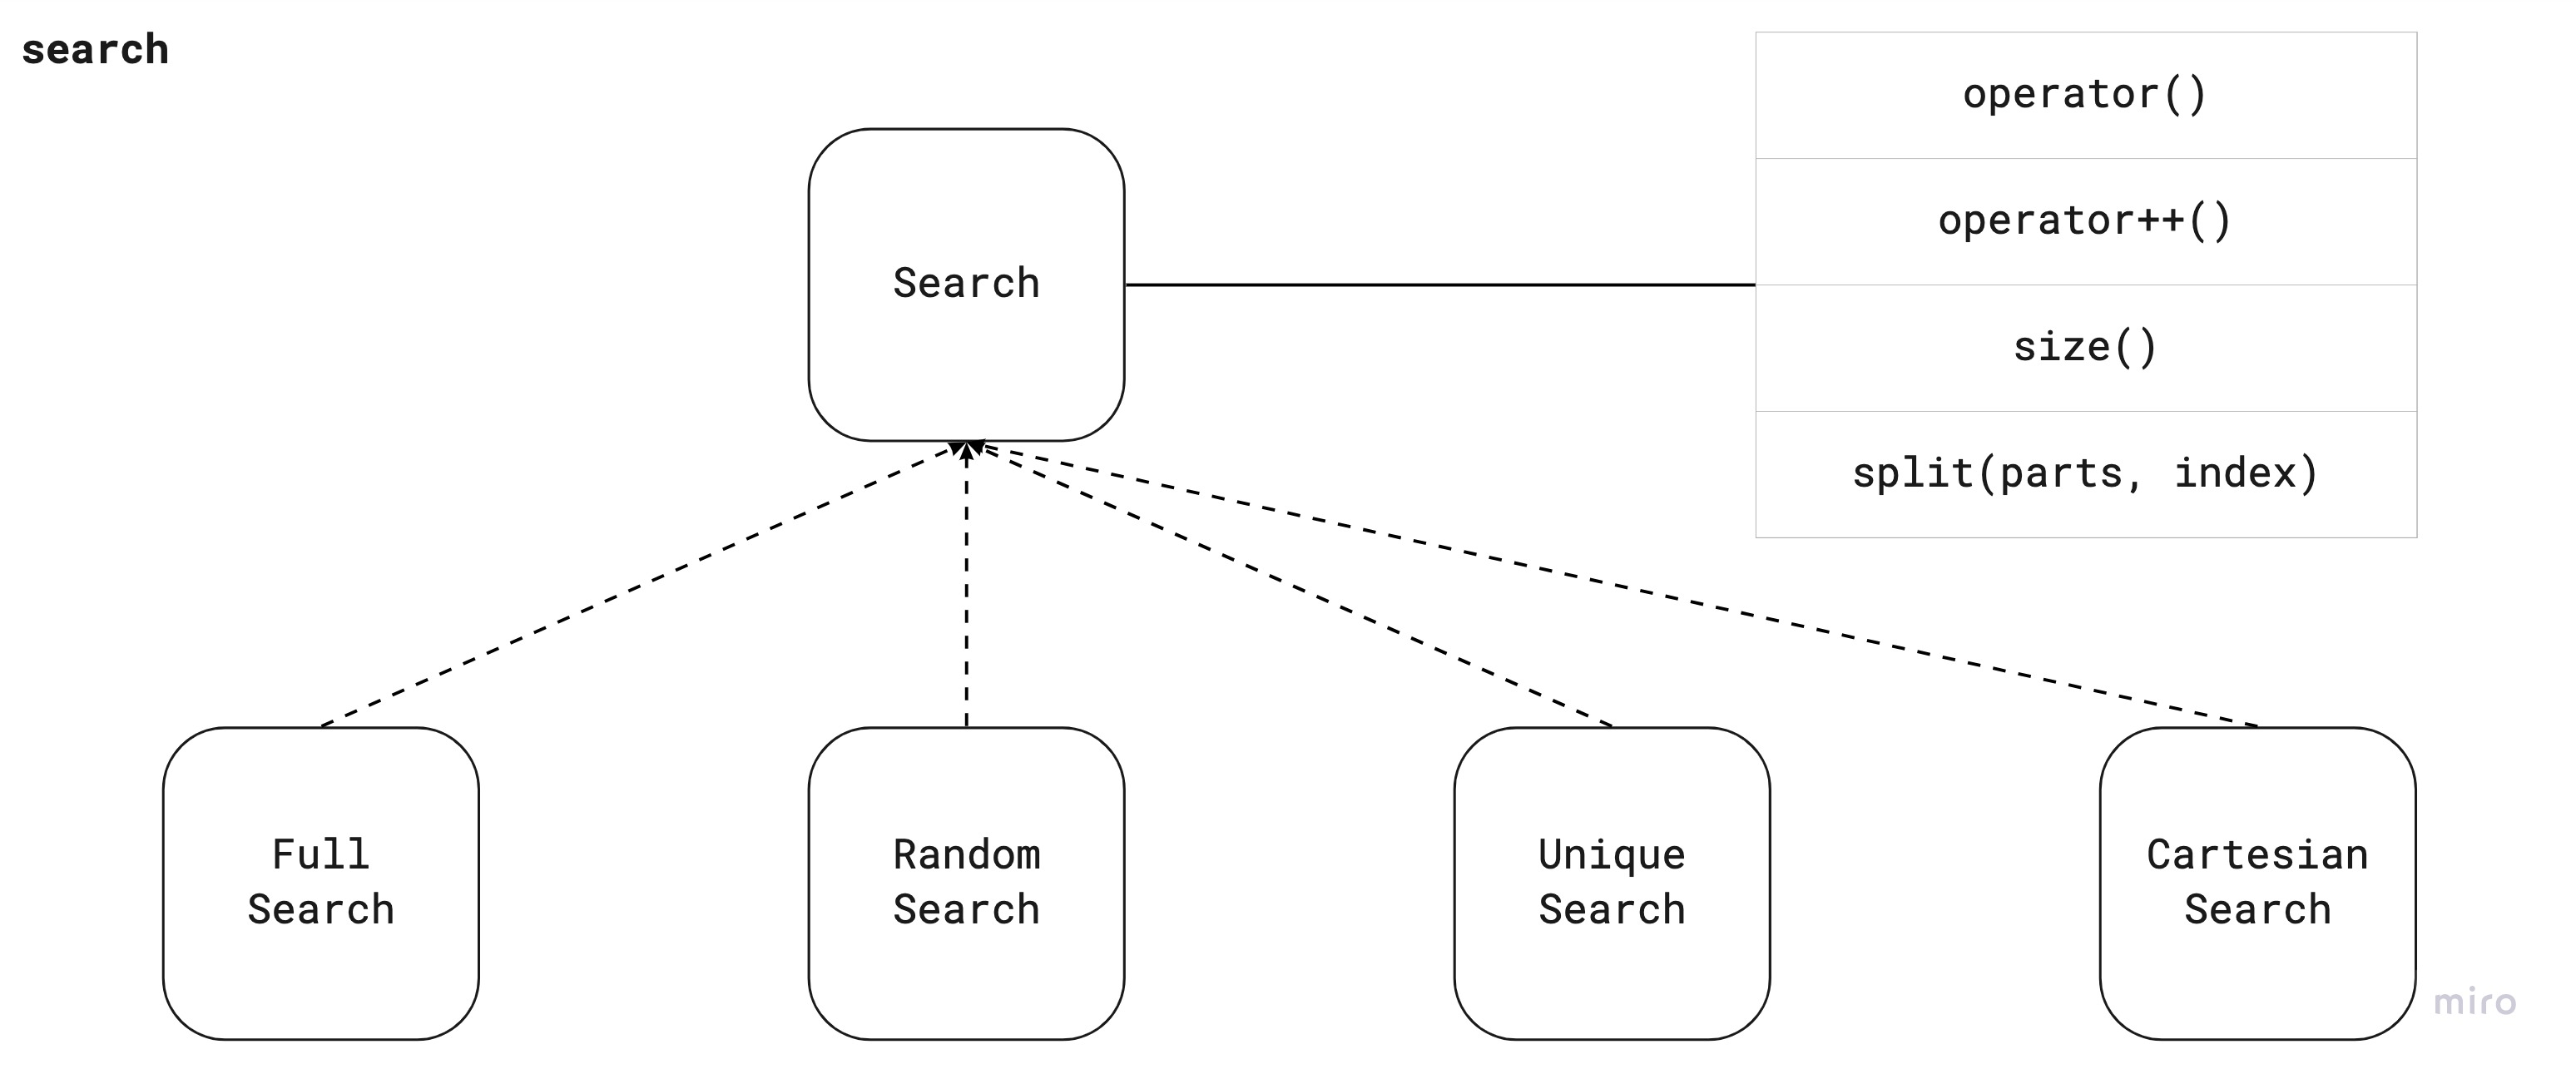
\includegraphics[width=\textwidth]{arch-search}
    \label{arch:rbs:prop:search-img}
\end{figure}

\begin{table}[H]
    \caption{Описание методов \textsc{Search}}\label{arch:rbs:prop:search-def}
    \centering
    \begin{tabularx}{\textwidth}{|*{3}{>{\centering\arraybackslash}X|}}\hline
        Метод & Параметры & Описание \\\hline
        \textsc{operator()} & -- & Возвращает текущий элемент выборки \\\hline
        \textsc{operator++} & -- & Переходит на следующий элемент выборки. Возвращает \textsc{false},
                                    если новый элемент -- последний \\\hline
        \textsc{size} & -- & Возвращает размер выборки \\\hline
        \textsc{split} & Число потоков, номер потока & Возвращает часть исходной выборки \\\hline
    \end{tabularx}
\end{table}

После получения выборки необходимо вызвать метод вывода последствий на всех элементах этой
выборки. Далее будут рассмотрены различные подходы к решению этой задачи: \textit{наивный
(последовательный), параллельный, вычисление $\rho$ через дерево поиска}.

\textit{Наивный подход}\label{arch:rbs:prop:naive}. Данный подход подразумевает последовательный
вызов метода вывода последствий. То есть, имея выборку $D$ и решатель $A$, значение $\rho$ 
аппроксимируется так, как показано в листинге \ref{arch:rbs:prop:naive-lst}.

\algdef{SE}[DOWHILE]{Do}{doWhile}{\algorithmicdo}[1]{\algorithmicwhile\ #1}%

\begin{algorithm}[H]
\caption{Наивное вычисление $\hat{\rho}$}\label{arch:rbs:prop:naive-lst}
\begin{algorithmic}
	\Function{calculate\_rho}{\textsc{A}, \textsc{D}}
        \State $S \leftarrow 0$
        \Do
            \State $\hat{b} \leftarrow \textsc{D()}$
            \If{\textsc{A($\hat{b}$)} = 0}
				\State $S \leftarrow S + 1$
			\EndIf
        \doWhile{\textsc{D++}}
        \State\Return $\frac{S}{N}$
	\EndFunction
\end{algorithmic}
\end{algorithm}

\textit{Параллельная обработка выборки}\label{arch:rbs:prop:par}. Данный подход разделяет выборку
на несколько выборок и обрабатывает их в разных потоках. Для этого используется метод \textsc{split}.
Псевдокод данного подхода представлен в листинге \ref{arch:rbs:prop:par-lst}.

\begin{algorithm}[H]
\caption{Параллельное вычисление $\hat{\rho}$}\label{arch:rbs:prop:par-lst}
\begin{algorithmic}
    \Function{calculate\_rho\_par}{$[\textsc{A}_i, i=\overline{1,M}]$, \textsc{D}}
        \State $S \leftarrow 0$
        \State $[\textsc{D}_i] \leftarrow \left[\textsc{D.split($M$, $j$),~ $j=\overline{1,M}$}\right]$
        \State\Return $\sum_{i}^{\textsc{parallel}}{\textsc{calculate\_rho($A_i$, $D_i$)}} / N$
	\EndFunction
\end{algorithmic}
\end{algorithm}

Данный подход с теоретической точки зрения крайне хорошо масштабируется, так как метод \textsc{split}
занимает несравнимо мало времени по сравнению с многократным вызовом метода вывода последствий. Практическое
сравнение последовательного и параллельного подходов приведено в Главе \ref{research:prop}.

\textit{Вычисление точного значения $\rho$ через дерево подстановок}\label{arch:rbs:prop:tree}.
Данный подход является новым и не имеет аналогов в известных мне решателях за ненадобностью. Однако,
идея, описанная далее, является крайне эффективной оптимизацией перебора $\hat{B}$, как показано в
Главе~\ref{research:prop}. Для вычисления точного значения $\rho$ необходимо посчитать число
подстановок $\hat{b} \in \hat{B}$, которые решаются заданным алгоритмом $A$. В данной работе, как
упомянуто ранее, в качестве этого алгоритма используется алгоритм вывода последствий. Результатом
работы этого алгоритма может быть либо информация о существовании конфликтующих подстановок переменных,
либо отсутствие дополнительной информации. Заметим, что если на каком-то префиксе $\hat{b}$ 
алгоритм сообщил о конфликте, то нет никакого смысла далее рассматривать подстановки с этим префиксом,
так как все они заведомо конфликтные. Можно просто прибавить к результату размер всего поддерева поиска.
Иллюстрация к данной идее приведена на рисунке \ref{arch:rbs:prop:tree-img}. Листинг, содержащий
псевдокод данного метода, приведен в приложении (листинг~\ref{append:rbs:prop:tree-lst}). Данный
метод был успешно реализован и встроен в исходный код решателя Minisat. Сравнительные результаты
с наивным и параллельным подходами содержатся в Главе~\ref{research:prop}.

\begin{figure}[H]
    \caption{Вычисление $\rho$ через дерево подстановок. Здесь $X,Y,Z$ --- переменные. Подстановки
    $E[X \mid 1]$ и $E[\{\,X,Y\,\} \mid \{\, X \to 0,~ Y \to 1 \,\}]$ приводят к конфликту, поэтому
    соответствующие поддеревья поиска можно не рассматривать.}
    \centering
    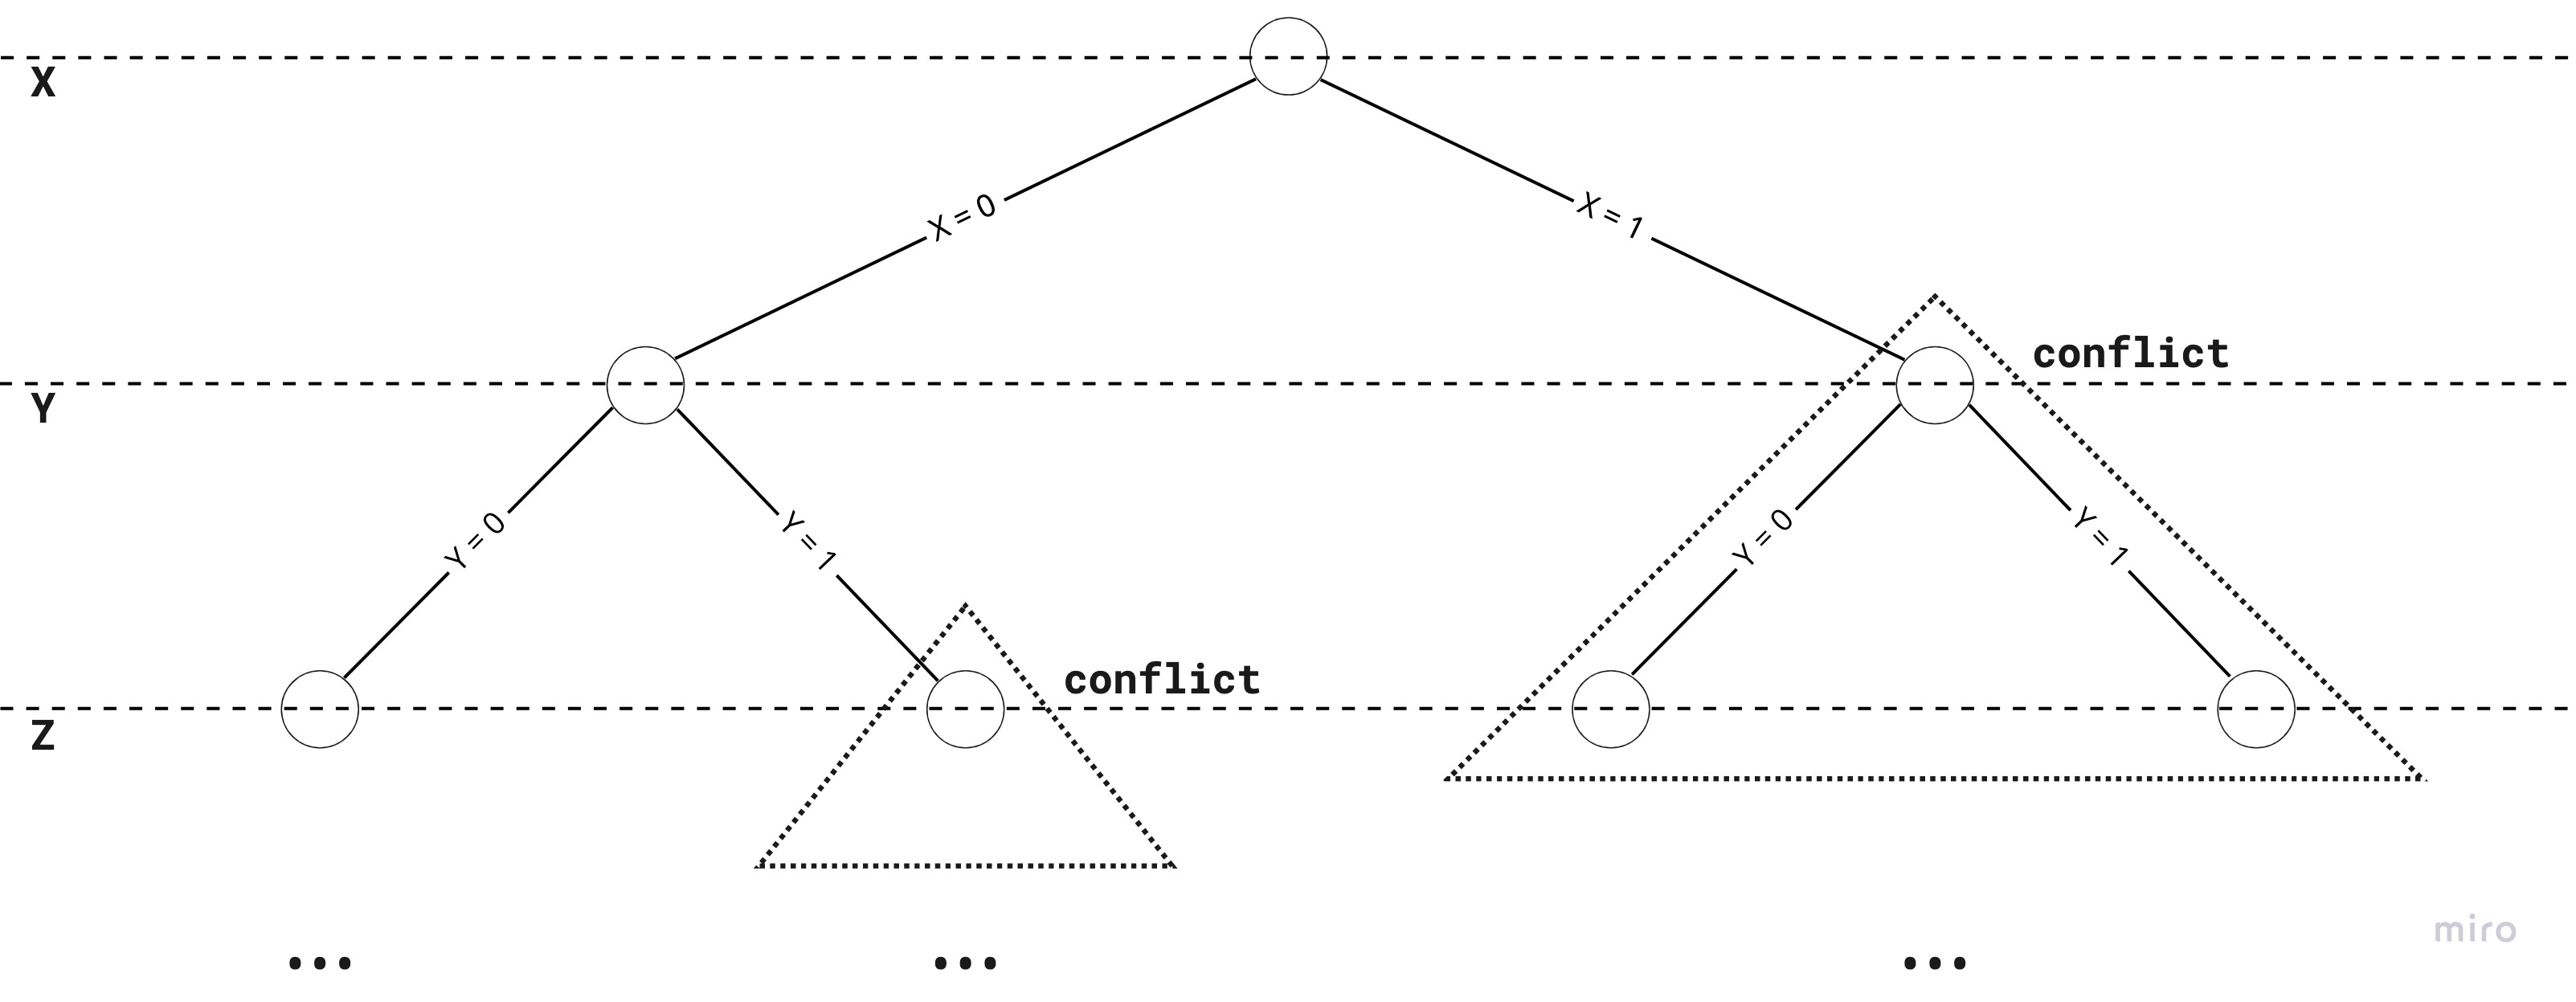
\includegraphics[width=\textwidth]{arch-tree}
    \label{arch:rbs:prop:tree-img}
\end{figure}

\section{Решение набора подстановок}\label{arch:solver}

В данной главе описана архитектура сервиса решения булевой функции с подстановками. Описан интерфейс
сервиса, приведена схема распределения задач по последовательным решателям, описана техника обмена
знаниями между решателями.

В качестве последовательных решателей используются Minisat~\cite{bib:minisat},
MapleCOMSPS~\cite{bib:maplecomsps}, painless-maplecomsps~\cite{bib:painless}. Под последовательным
имеется в виду не тип самого решателя, а невозможность параллельного решения разных задач.
То есть, painless-mcomsps является параллельным решателем, но может решать лишь одну задачу
одновременно. Описываемый сервис нужен именно для того, чтобы обеспечить возможность параллельного 
решения разных задач, что необходимо для реализации параллельных алгоритмов решения на основе 
подхода разделяй-и-властвуй~\ref{overview:dac}.

Схема наследования интерфейса \textsc{SolverService} проиллюстрирована на рисунке~\ref{arch:solver:serv-img}.
Описание методов интерфейса приведено в таблице~\ref{arch:solver:serv-def}.

\begin{figure}[H]
    \caption{Интерфейс \textsc{SolverService} и его реализация}
    \centering
    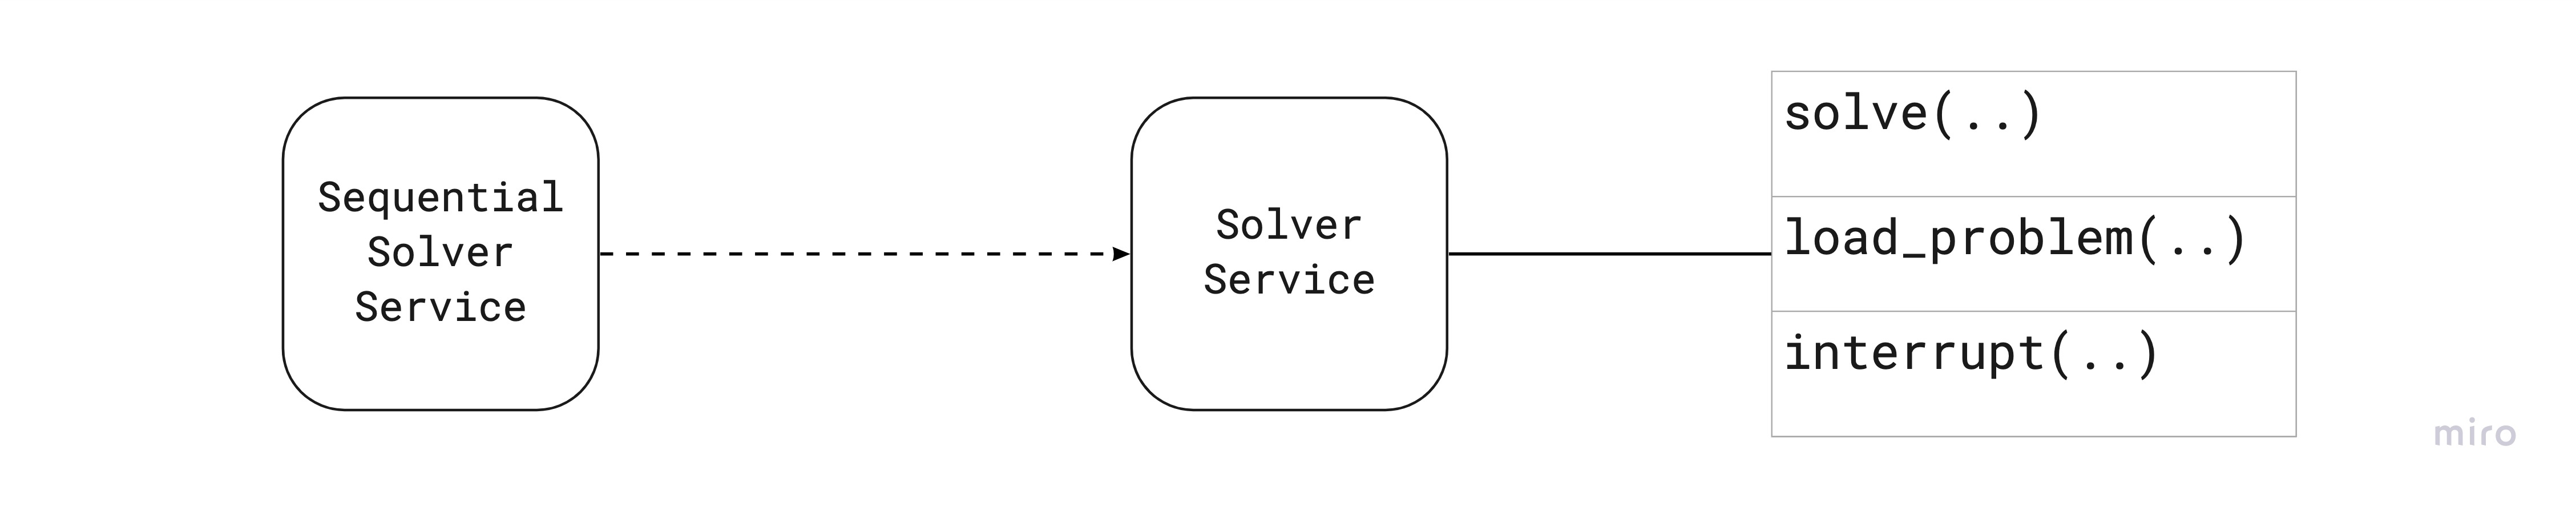
\includegraphics[width=\textwidth]{arch-solver}
    \label{arch:solver:serv-img}
\end{figure}

\begin{table}[H]
    \caption{Описание методов \textsc{SolverService}}\label{arch:solver:serv-def}
    \centering
    \begin{tabularx}{\textwidth}{|*{3}{>{\centering\arraybackslash}X|}}\hline
        Метод & Параметры & Описание \\\hline
        \textsc{solve} & Подстановка, ограничение по времени, callback-функция, вызываемая 
                        при окончании решения & Возвращает объект \textsc{std::future} типизированный
                        результатом решения, и добавляет задачу в очередь \\\hline
        \textsc{load\_problem} & -- & Загружает формулу в решатель \\\hline
        \textsc{interrupt} & -- & Прерывает процесс решения \\\hline
    \end{tabularx}
\end{table}

Реализация \textsc{SequentialSolverService} управляет набором последовательных решателей, работающих
параллельно: обеспечивает их задачами, а также, при необходимости, обеспечивает обмен знаниями.
Для распределения задач реализована безопасная для использования в многопоточной среде очередь.
Для обмена знаниями используются механизмы, реализованные в интерфейсе \textsc{painless} и адаптированные
для использования разных решателей и схем обмена. Схема работы \textsc{SequentialSolverService}
приведена на рисунке~\ref{arch:solver:seq-img}.

\begin{figure}[H]
    \caption{Схема работы \textsc{SequentialSolverService}}
    \centering
    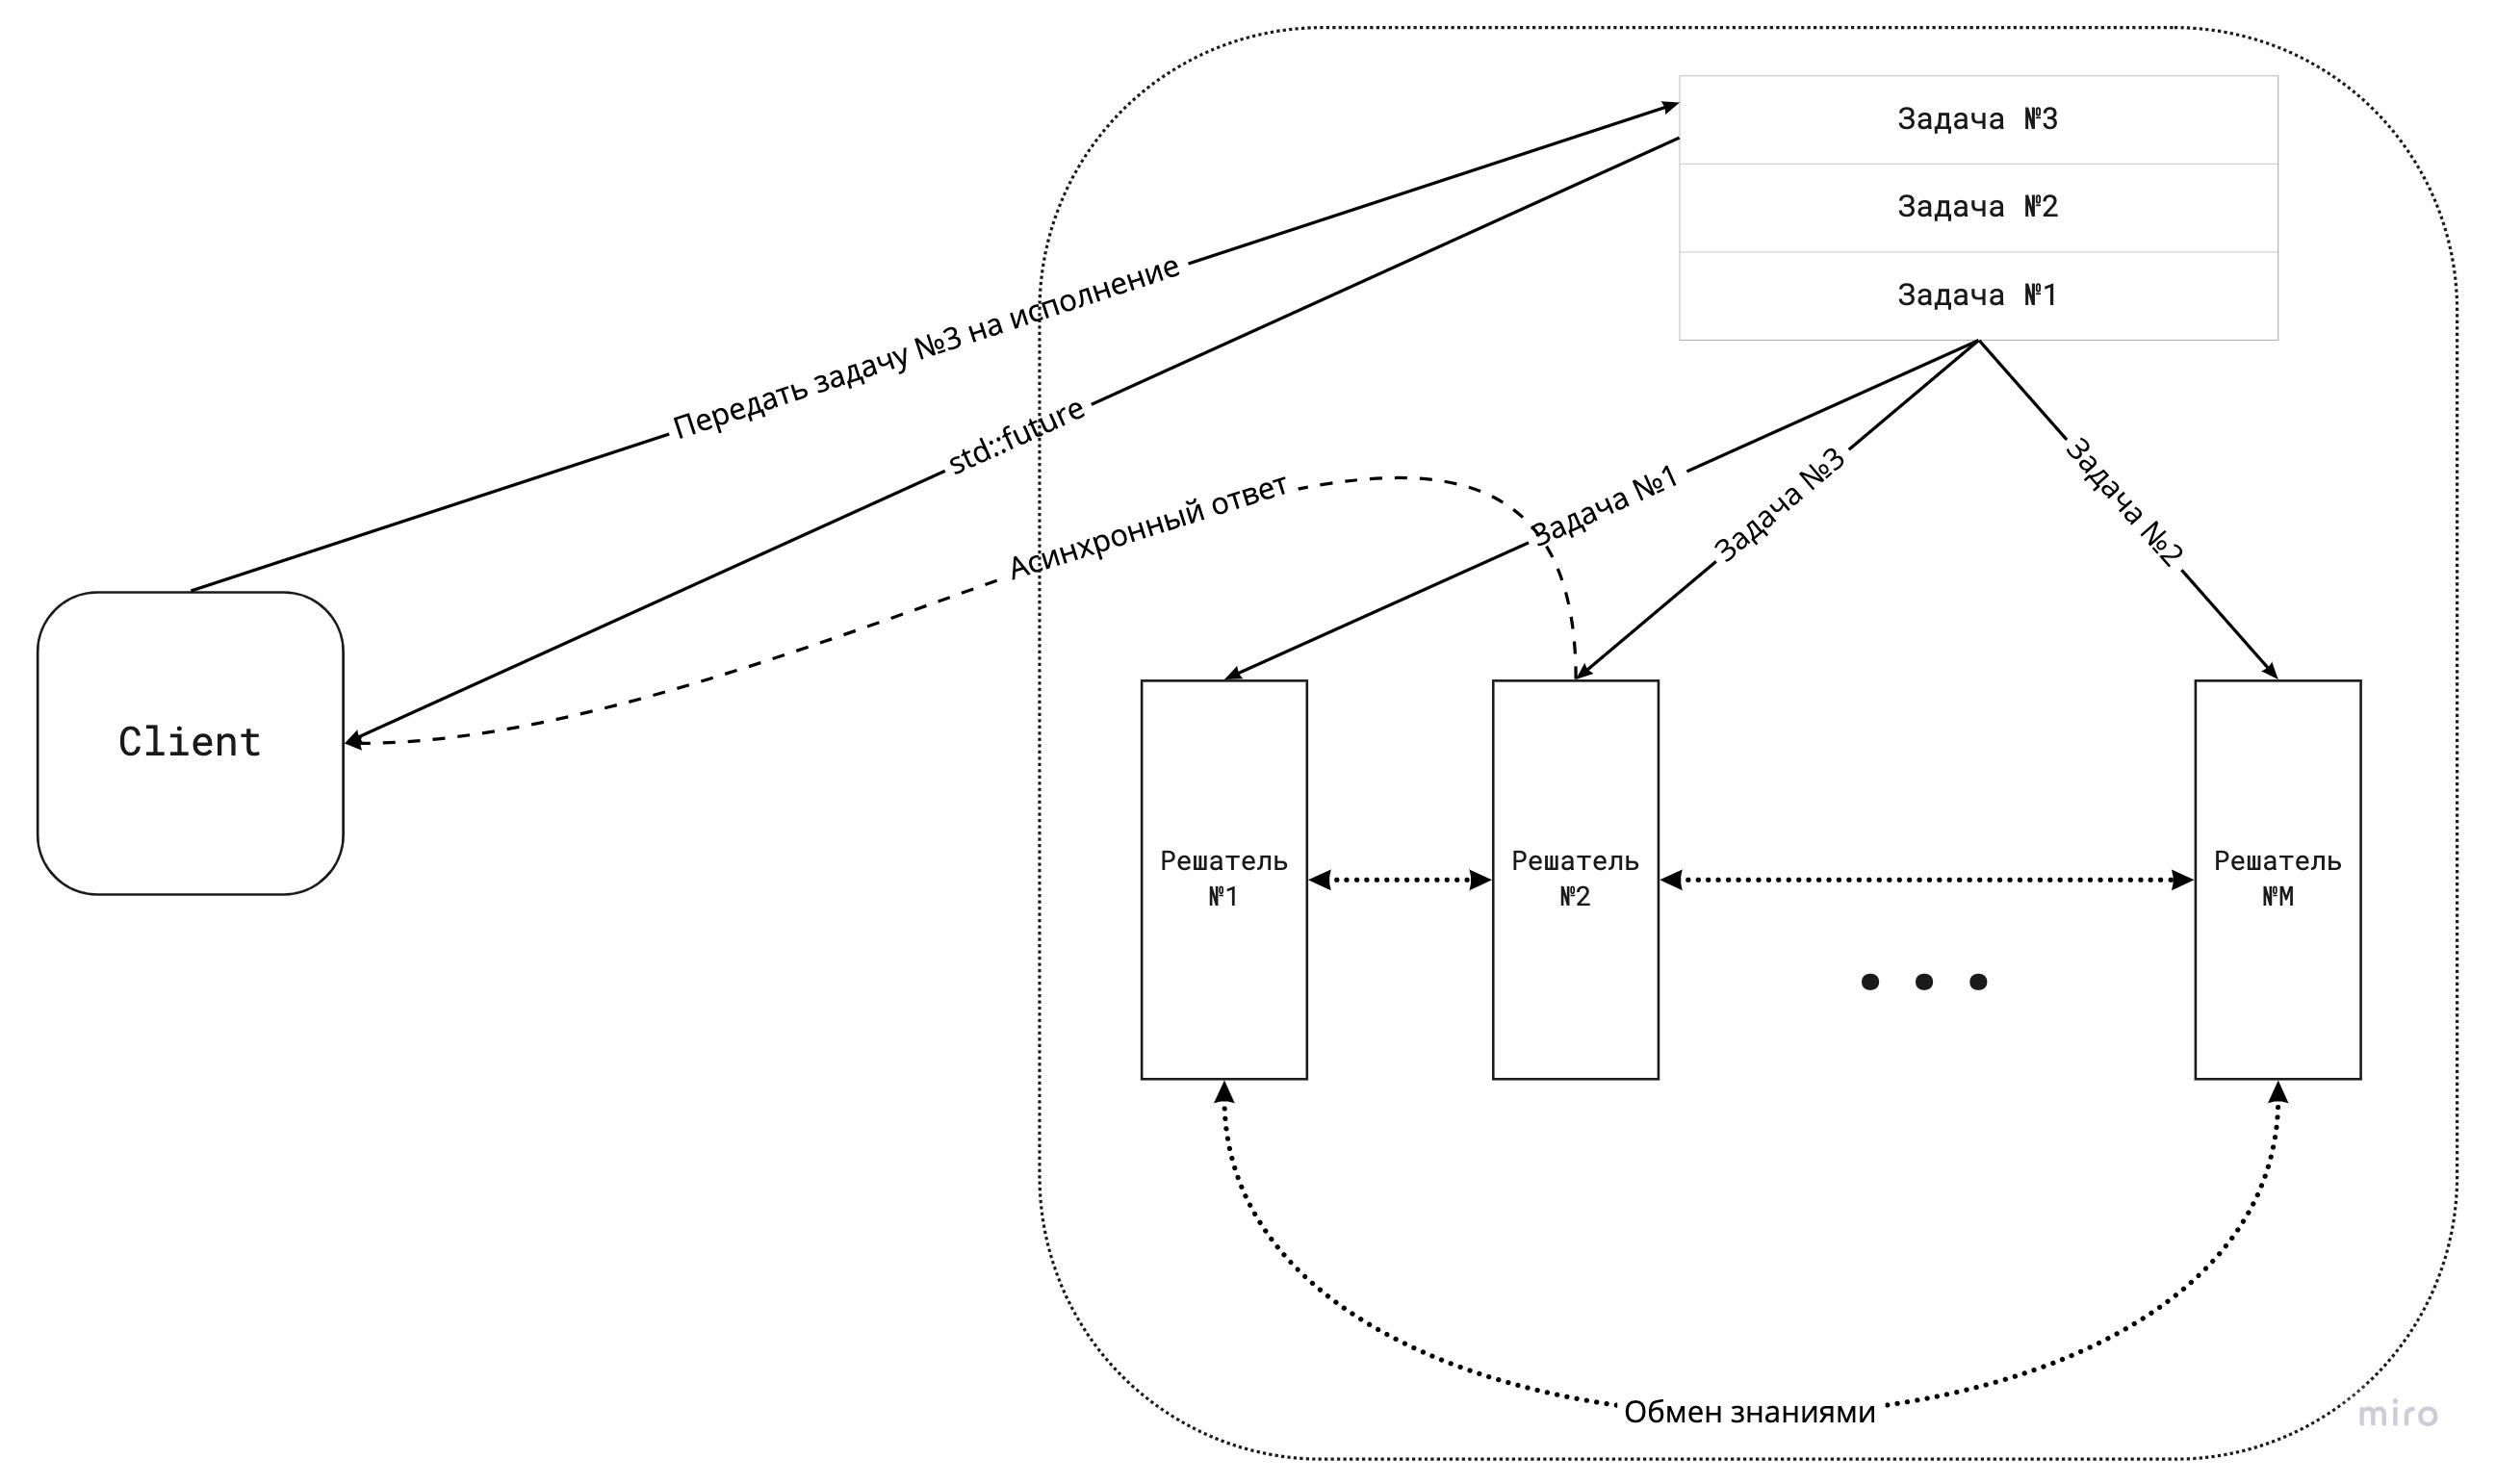
\includegraphics[width=\textwidth]{arch-seq}
    \label{arch:solver:seq-img}
\end{figure}

\section{Использование вероятностных лазеек}\label{arch:solve}

В данной главе описаны реализованные подходы к использованию вероятностных лазеек для решения
задач булевой выполнимости. Описаны \textit{прямой} и \textit{рекурсивный} подоходы к решению,
а также схема с \textit{использованием нескольких лазеек}.

\section{Описание реализации}\label{arch:impl}

В данной главе описана структура исходного кода алгоритма, перечислены возможные опции как при
сборке, так и при запуске приложения.

\chapterconclusion
